\documentclass{beamer}

% xcolor and define colors -------------------------
\usepackage{xcolor}

% https://www.viget.com/articles/color-contrast/
\definecolor{purple}{HTML}{5601A4}
\definecolor{navy}{HTML}{0D3D56}
\definecolor{ruby}{HTML}{9a2515}
\definecolor{alice}{HTML}{107895}
\definecolor{daisy}{HTML}{EBC944}
\definecolor{coral}{HTML}{F26D21}
\definecolor{kelly}{HTML}{829356}
\definecolor{cranberry}{HTML}{E64173}
\definecolor{jet}{HTML}{131516}
\definecolor{asher}{HTML}{555F61}
\definecolor{slate}{HTML}{314F4F}

% Mixtape Sessions
\definecolor{picton-blue}{HTML}{00b7ff}
\definecolor{violet-red}{HTML}{ff3881}
\definecolor{sun}{HTML}{ffaf18}
\definecolor{electric-violet}{HTML}{871EFF}

% Main theme colors
\definecolor{accent}{HTML}{00b7ff}
\definecolor{accent2}{HTML}{871EFF}
\definecolor{gray100}{HTML}{f3f4f6}
\definecolor{gray800}{HTML}{1F292D}


% Beamer Options -------------------------------------

% Background
\setbeamercolor{background canvas}{bg = white}

% Change text margins
\setbeamersize{text margin left = 15pt, text margin right = 15pt} 

% \alert
\setbeamercolor{alerted text}{fg = accent2}

% Frame title
\setbeamercolor{frametitle}{bg = white, fg = jet}
\setbeamercolor{framesubtitle}{bg = white, fg = accent}
\setbeamerfont{framesubtitle}{size = \small, shape = \itshape}

% Block
\setbeamercolor{block title}{fg = white, bg = accent2}
\setbeamercolor{block body}{fg = gray800, bg = gray100}

% Title page
\setbeamercolor{title}{fg = gray800}
\setbeamercolor{subtitle}{fg = accent}

%% Custom \maketitle and \titlepage
\setbeamertemplate{title page}
{
    %\begin{centering}
        \vspace{20mm}
        {\Large \usebeamerfont{title}\usebeamercolor[fg]{title}\inserttitle}\\
        {\large \itshape \usebeamerfont{subtitle}\usebeamercolor[fg]{subtitle}\insertsubtitle}\\ \vspace{10mm}
        {\insertauthor}\\
        {\color{asher}\small{\insertdate}}\\
    %\end{centering}
}

% Table of Contents
\setbeamercolor{section in toc}{fg = accent!70!jet}
\setbeamercolor{subsection in toc}{fg = jet}

% Button 
\setbeamercolor{button}{bg = accent}

% Remove navigation symbols
\setbeamertemplate{navigation symbols}{}

% Table and Figure captions
\setbeamercolor{caption}{fg=jet!70!white}
\setbeamercolor{caption name}{fg=jet}
\setbeamerfont{caption name}{shape = \itshape}

% Bullet points

%% Fix left-margins
\settowidth{\leftmargini}{\usebeamertemplate{itemize item}}
\addtolength{\leftmargini}{\labelsep}

%% enumerate item color
\setbeamercolor{enumerate item}{fg = accent}
\setbeamerfont{enumerate item}{size = \small}
\setbeamertemplate{enumerate item}{\insertenumlabel.}

%% itemize
\setbeamercolor{itemize item}{fg = accent!70!white}
\setbeamerfont{itemize item}{size = \small}
\setbeamertemplate{itemize item}[circle]

%% right arrow for subitems
\setbeamercolor{itemize subitem}{fg = accent!60!white}
\setbeamerfont{itemize subitem}{size = \small}
\setbeamertemplate{itemize subitem}{$\rightarrow$}

\setbeamertemplate{itemize subsubitem}[square]
\setbeamercolor{itemize subsubitem}{fg = jet}
\setbeamerfont{itemize subsubitem}{size = \small}







% Links ----------------------------------------------

\usepackage{hyperref}
\hypersetup{
  colorlinks = true,
  linkcolor = accent2,
  filecolor = accent2,
  urlcolor = accent2,
  citecolor = accent2,
}


% Line spacing --------------------------------------
\usepackage{setspace}
\setstretch{1.2}


% \begin{columns} -----------------------------------
\usepackage{multicol}


% Fonts ---------------------------------------------
% Beamer Option to use custom fonts
\usefonttheme{professionalfonts}

% \usepackage[utopia, smallerops, varg]{newtxmath}
% \usepackage{utopia}
\usepackage[sfdefault,light]{roboto}

% Small adjustments to text kerning
\usepackage{microtype}



% Remove annoying over-full box warnings -----------
\vfuzz2pt 
\hfuzz2pt


% Table of Contents with Sections
\setbeamerfont{myTOC}{series=\bfseries, size=\Large}
\AtBeginSection[]{
        \frame{
            \frametitle{Roadmap}
            \tableofcontents[current]   
        }
    }


% Tables -------------------------------------------
% Tables too big
% \begin{adjustbox}{width = 1.2\textwidth, center}
\usepackage{adjustbox}
\usepackage{array}
\usepackage{threeparttable, booktabs, adjustbox}
    
% Fix \input with tables
% \input fails when \\ is at end of external .tex file
\makeatletter
\let\input\@@input
\makeatother

% Tables too narrow
% \begin{tabularx}{\linewidth}{cols}
% col-types: X - center, L - left, R -right
% Relative scale: >{\hsize=.8\hsize}X/L/R
\usepackage{tabularx}
\newcolumntype{L}{>{\raggedright\arraybackslash}X}
\newcolumntype{R}{>{\raggedleft\arraybackslash}X}
\newcolumntype{C}{>{\centering\arraybackslash}X}

% Figures

% \imageframe{img_name} -----------------------------
% from https://github.com/mattjetwell/cousteau
\newcommand{\imageframe}[1]{%
    \begin{frame}[plain]
        \begin{tikzpicture}[remember picture, overlay]
            \node[at = (current page.center), xshift = 0cm] (cover) {%
                \includegraphics[keepaspectratio, width=\paperwidth, height=\paperheight]{#1}
            };
        \end{tikzpicture}
    \end{frame}%
}

% subfigures
\usepackage{subfigure}


% Highlight slide -----------------------------------
% \begin{transitionframe} Text \end{transitionframe}
% from paulgp's beamer tips
\newenvironment{transitionframe}{
    \setbeamercolor{background canvas}{bg=accent!40!black}
    \begin{frame}\color{accent!10!white}\LARGE\centering
}{
    \end{frame}
}


% Table Highlighting --------------------------------
% Create top-left and bottom-right markets in tabular cells with a unique matching id and these commands will outline those cells
\usepackage[beamer,customcolors]{hf-tikz}
\usetikzlibrary{calc}
\usetikzlibrary{fit,shapes.misc}

% To set the hypothesis highlighting boxes red.
\newcommand\marktopleft[1]{%
    \tikz[overlay,remember picture] 
        \node (marker-#1-a) at (0,1.5ex) {};%
}
\newcommand\markbottomright[1]{%
    \tikz[overlay,remember picture] 
        \node (marker-#1-b) at (0,0) {};%
    \tikz[accent!80!jet, ultra thick, overlay, remember picture, inner sep=4pt]
        \node[draw, rectangle, fit=(marker-#1-a.center) (marker-#1-b.center)] {};%
}

\usepackage{breqn} % Breaks lines

\usepackage{amsmath}
\usepackage{mathtools}

\usepackage{pdfpages} % \includepdf

\usepackage{listings} % R code
\usepackage{verbatim} % verbatim

% Video stuff
\usepackage{media9}

% packages for bibs and cites
\usepackage{natbib}
\usepackage{har2nat}
\newcommand{\possessivecite}[1]{\citeauthor{#1}'s \citeyearpar{#1}}
\usepackage{breakcites}
\usepackage{alltt}

% tikz
\usepackage{tikz}
\usepackage{pgfplots}
\usetikzlibrary{calc, positioning, decorations.pathreplacing, arrows.meta, intersections}
\pgfdeclarelayer{bg}
\pgfdeclarelayer{back}
\pgfdeclarelayer{fg}
\pgfsetlayers{bg,main,fg,back}
\usetikzlibrary{shapes,arrows}

% Setup math operators
\DeclareMathOperator{\E}{E} \DeclareMathOperator{\tr}{tr} \DeclareMathOperator{\se}{se} \DeclareMathOperator{\I}{I} \DeclareMathOperator{\sign}{sign} \DeclareMathOperator{\supp}{supp} \DeclareMathOperator{\plim}{plim}
\DeclareMathOperator*{\dlim}{\mathnormal{d}\mkern2mu-lim}
\newcommand\independent{\protect\mathpalette{\protect\independenT}{\perp}}
   \def\independenT#1#2{\mathrel{\rlap{$#1#2$}\mkern2mu{#1#2}}}
\newcommand*\colvec[1]{\begin{pmatrix}#1\end{pmatrix}}

\newcommand{\myurlshort}[2]{\href{#1}{\textcolor{gray}{\textsf{#2}}}}


\begin{document}



% ---- Content ----

% 20 min. no more than 20 slides (15 ideally). The goal is to keep the audience's attention 

% 7 min of causal inference as a methodology
% advances in this line of work --> more specific impact assessment
% 10 min commenting on the study, the type of assessment that took place
% "based on what I've seen, Causal Infernce in its newest version, it can give more room for answering questions about impact of programs".  Position causal inference within the impact evaluation methodology.  It can do "1 2 3 4 5" and then show examples.  First 10 minutes.  

% goal: to formulate a program (expensive currently to Egyptian government).  We need to know the proper assessment.  Are the methodologies proper enough to justify how much money is being spent? 
% my advantage is that I am an outsider; I'm watching it but talking about it from my own expertise.
% Other panelists will speak about the study they undertook.  We want to know what they are doing -- everyone is involved in the assessment (JPAL, for instance).  Some of the panelists will be critical (e.g., an anthropologist may be critical).  I can use examples.  But use examples to illustrate the methodologies using benign topics that aren't offensive or polarizing.  
% What can be done with quasi-experimental methodologies versus what I have seen being assessed.  I want to open doors.  They're going to put in a proposal for an assessment of the program. 

% Can I discuss "treatment assignment mechanism" but without so much detail?  And can I drop the potential outcomes material and just assume the average treatment effect. 

% Be critical of the study, say what I think what kinds of improvements can be done.  

% I won't need to explain the program as that'll be described before my talk.  Go into an assessment of its impact. Cost benefit is important for normative questions.

% Use as a thread the program so that I wrap people into this idea.  

% Common errors for conclusions for not understanding.  I need entry points for grabbing people. 

\section{What is causal inference?}



\subsection{Core questions in causal inference}


%\begin{frame}{Introduction: About Me}
%\begin{itemize}
%\item I'm Scott Cunningham, the Ben H. Williams Professor of Economics at Baylor University
%\item Baylor is located in Waco, Texas: a small city in one of the USA's largest states by area and population.
%\item I'm the author of \underline{Causal Inference: the Mixtape}, as well as numerous articles in applied economics focusing on gender, crime, maternal health, drug policy, and mental illness and self harm in prisons and jails
%\item I'm honored and appreciative to be here with you all today.
%\end{itemize}
%\end{frame}

\begin{frame}{Overview of Today's Talk}
\begin{itemize}
\item Firstly, we'll explore \emph{causal inference}: 
    \begin{itemize}
    \item What is it?  Why is it important?  What is at stake? % what is the value added of the techniques in causal inference and what are examples of assessment. I need to use the 10 minutes to make the point for causal inference -- focusing on the range of methods. 
    \item Emphasizing the importance of \emph{controlled randomization} and options when that fails.
    \end{itemize}
\item Secondly, we'll delve into a recent evaluation by Breisinger and coauthors:
    \begin{itemize}
    \item Focusing on the Takaful (Solidarity) and Karama (Dignity) programs.
    \item Understanding the evaluation's findings and implications.
    \end{itemize}
\end{itemize}
\end{frame}


\begin{frame}{Important Distinctions: Causality vs. Causal Inference}

What is causal inference?  What is causality?  They are related but not the same thing. 

\bigskip

\begin{itemize}
\item \emph{Causality} is a metaphysical concept which is stored within the branch of philosophy focusing on the nature of reality
\item \emph{Causal Inference} is an epistemological concept which is stored within the branch of philosophy focused on the nature of knowledge and beliefs
\end{itemize}
\end{frame}


\begin{frame}{Important Distinctions: Correlation vs. Causal Inference}

What is correlation?  When is it causal and when is it not? 

\bigskip

\begin{itemize}
\item \emph{Correlation} is a purely statistical concept measuring movements between two things
\item \emph{Causal Inference} cuts into the causal relationships in data using credible methods
\end{itemize}
\end{frame}

\begin{frame}{Causal Inference Gains}

\begin{itemize}

\item What do we gain from the developments in causal inference?
\item Discuss the advantages and the costs of not adopting it

\end{itemize}
\end{frame}


%\begin{frame}{Metaphysics of Causality}
%\begin{itemize}
%\item Metaphysics is the study of what exists and the nature of that existence
%\item The metaphysics of causality seeks to define what it means for one event to cause another
%\item Explores the fundamental nature of the causal relationship
%\item Poses questions like: "What does it mean, fundamentally, for A to cause B?"
%\end{itemize}
%\end{frame}

%\begin{frame}{Epistemology of Causal Inference}
%\begin{itemize}
%\item Epistemology is the study of how we know what we know.
%\item The epistemology of causal inference focuses on how we infer causal relationships, or what it means for a causal belief to be credible
%\item Causal inference is focused on building useful methods that can be relied on to infer one thing caused another, as opposed to philosophical inquiries into the nature of reality
%\item We ask: "How can we reliably infer that our social programs caused the lives of poor people to improve?"
%\end{itemize}
%\end{frame}


\begin{frame}{Common errors}

  \begin{itemize}
    \item Aliens from another planet come and notice that people on ventilators have higher mortality than those not on ventilators
    \item They conclude that ventilators are killing people
    \item Are they right?  Or  they have it backwards -- maybe doctors are putting sick people on ventilators to help them
    \item How can separate the two?  By understanding the behaviors that drove people into and out of programs first and combining that with statistical methodologies that take advantage of that
  \end{itemize}

\end{frame}

\begin{frame}{\#1: Correlation and causality are different concepts}

  \begin{itemize}
  	\item Differences between causality and correlation
		\begin{itemize}
	    \item Causal is about understanding the effect of one unit changing on another. ``If a person  puts a patient on a ventilator, will her covid symptoms improve?''
	    \item Correlation, on the other hand, is about understanding relationships across many units. ``How do changes in ventilators relate to changes in covid symptoms across a population?''
	    	\end{itemize}
	\item Failure to understand the difference between causal inference and \emph{description} can lead to major errors in assessment and therefore policy recommendations
  \end{itemize}  
\end{frame}



\begin{frame}{\#2: Coming first may not mean causality!}

  \begin{itemize}
    \item Every morning the rooster crows and then the sun rises
    \item Did the rooster cause the sun to rise? Or did the sun cause the rooster to crow?
    \item What if cat killed the rooster?  Would the sun never rise?
    \item Simply assuming things happening one after another represents causal effects is an extension of the previous error
  \end{itemize}

\end{frame}

\begin{frame}{\#3: Causality may mask correlations!}

  \begin{figure}
    \centering
    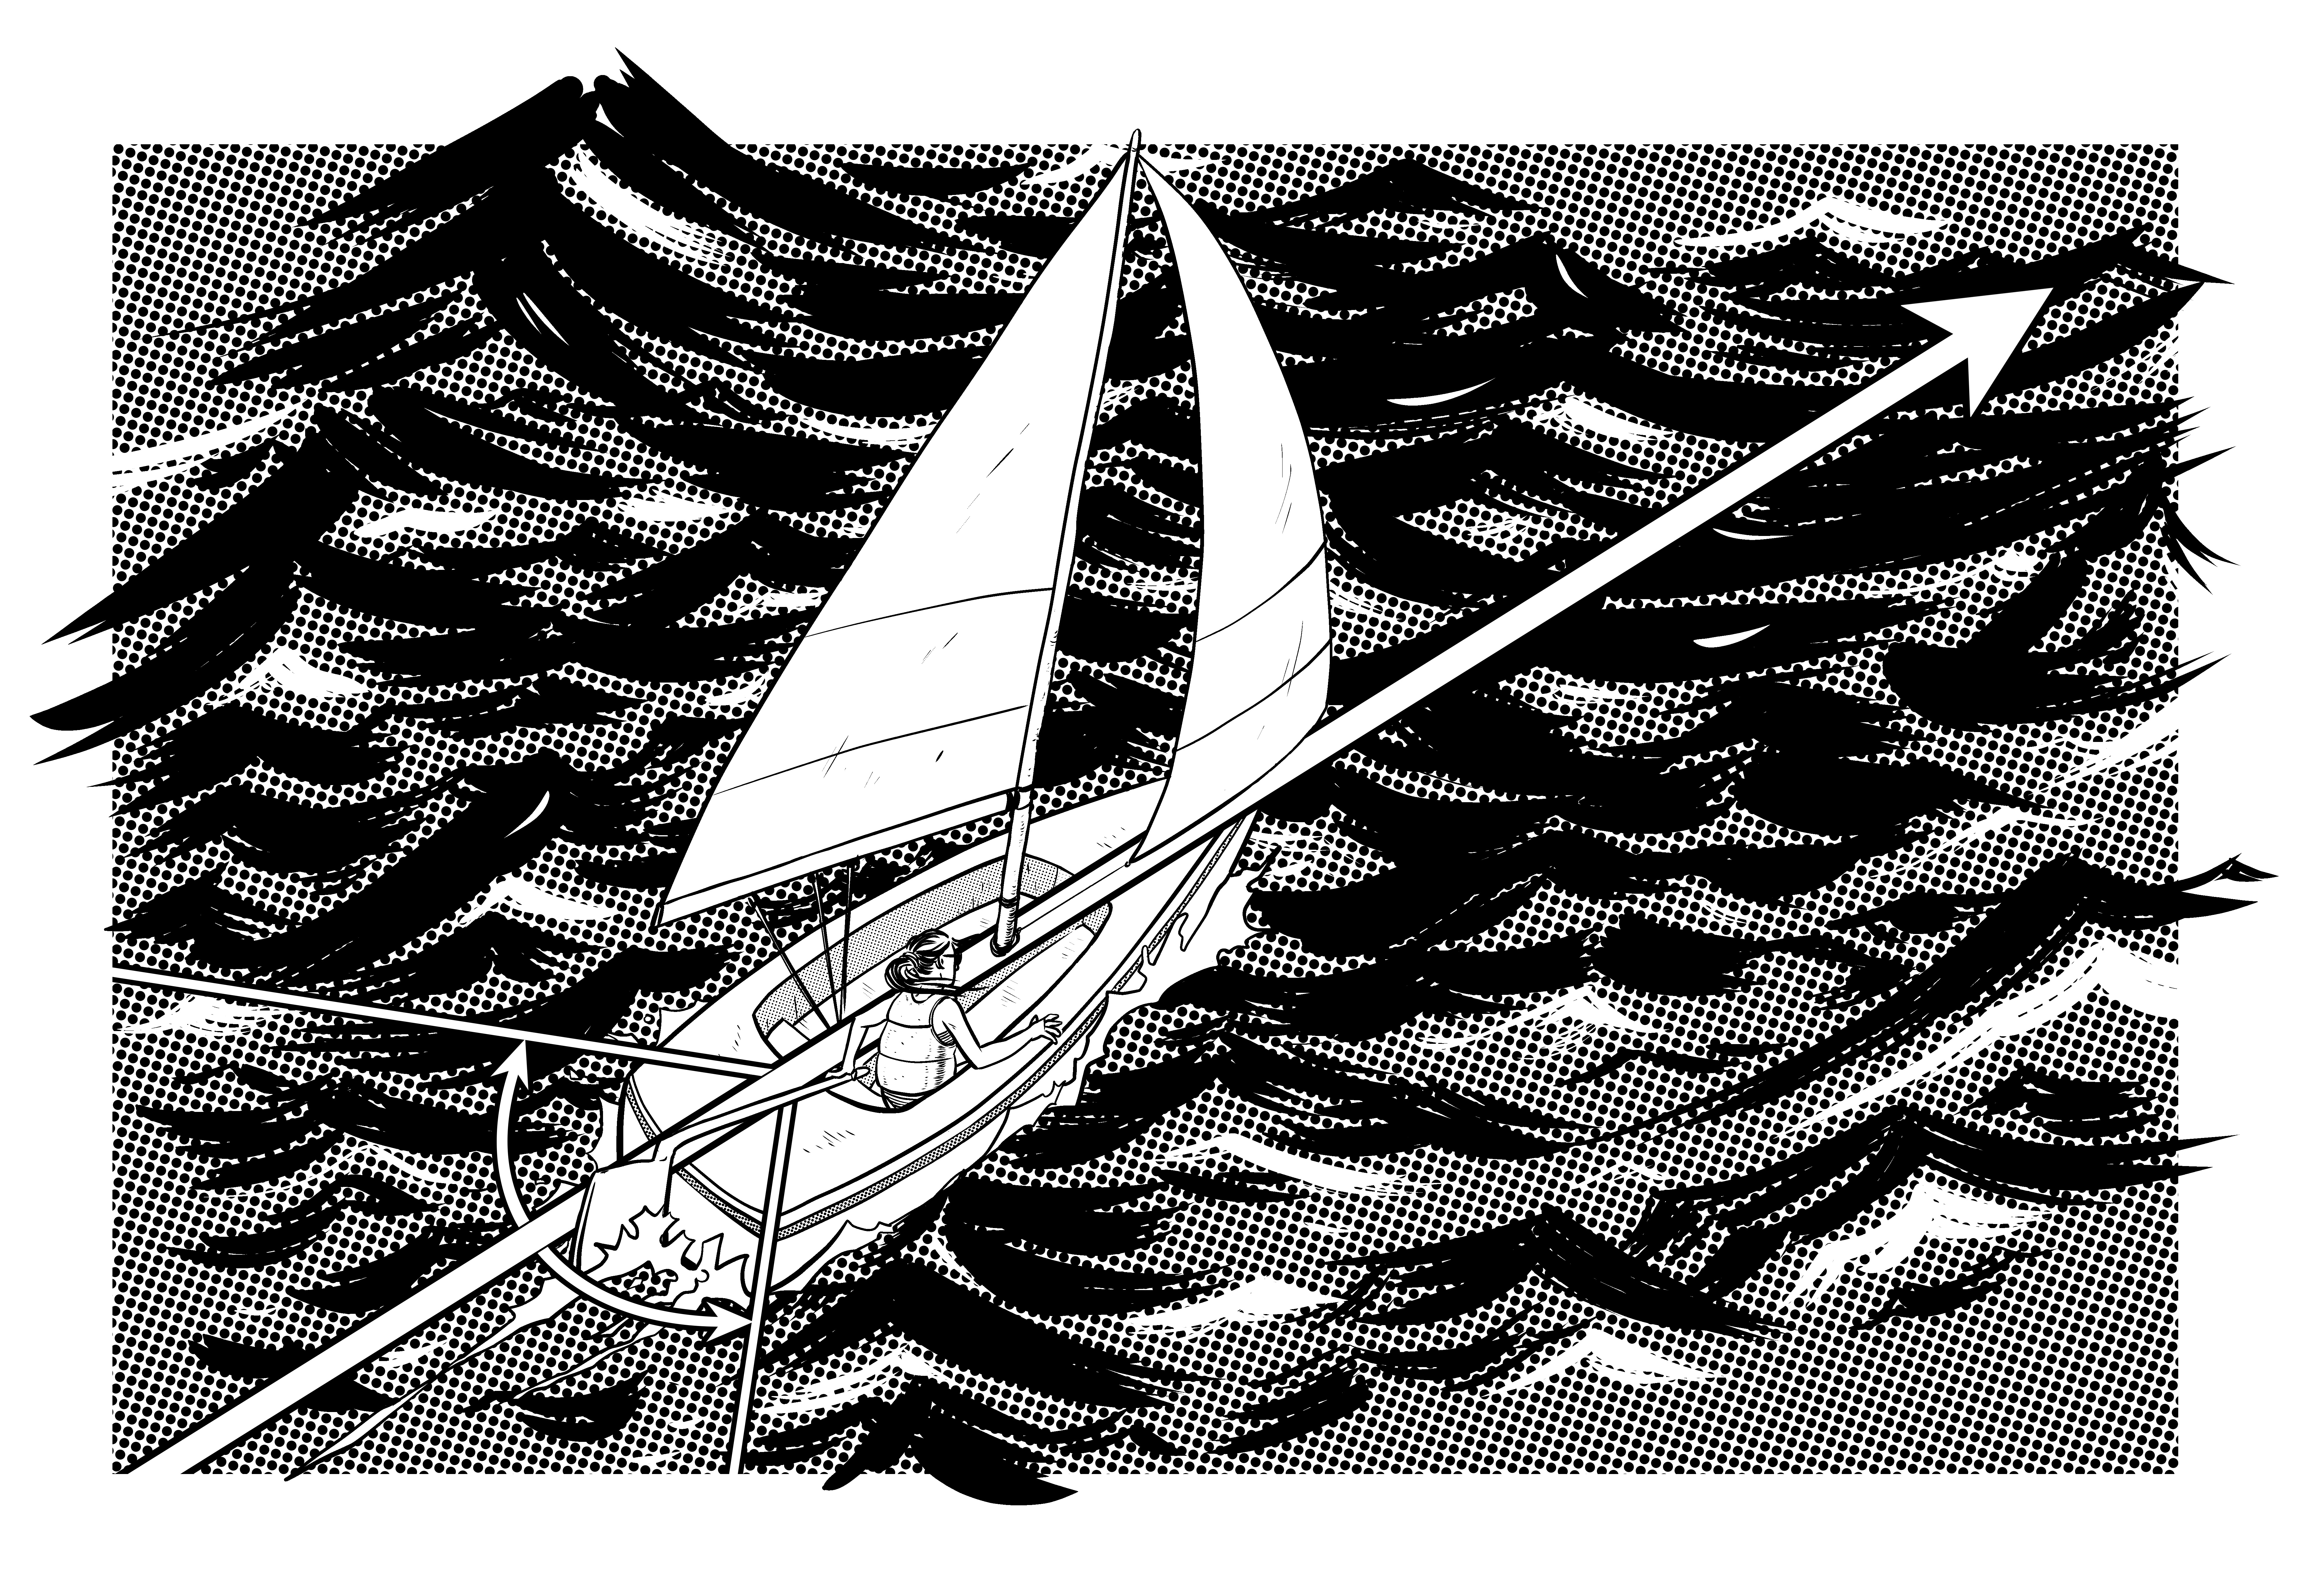
\includegraphics[scale=0.04]{./lecture_includes/scottboat.jpg}
  \end{figure}

\end{frame}

\subsection{Treatment Assignment Mechanisms}


%\begin{frame}{Three New Ideas}

%\begin{enumerate}
%\item \textbf{Counterfactual}: Philosophers come to it first and its central role in causal inference makes causality \emph{unknowable} that the project is nearly derailed
%\item \textbf{Treatment assignment mechanism}: Neyman and Fisher solve the counterfactual problem in statistics and lay the foundation of the modern randomized controlled trial (RCT) %with their focus on the selection process
%\item \textbf{No One Causal Effect}: There is no such thing as ``the causal effect''; there's many and your first step is to pick a parameter (not as easy as it sounds)
%\end{enumerate}


%\end{frame}

\begin{frame}{Correlations, Causal Effects, and Selection Bias}

\begin{itemize}
\item Comparing any two groups to one another has two main components:
	\begin{enumerate}
	\item \textbf{Average causal effect}: What is the average effect of the Takaful  and Karama programs on nutrition?
	\item \textbf{Selection bias}: How much of the observed differences between program participants is due to differences between them that would've existed regardless if they were on the program
	\end{enumerate}
\item Causal inference goal is to find a reason where we can believe there is no selection bias, and to do that we need to understand why people got into the program in the first place

\end{itemize}

\end{frame}


% Rewrite this but without the equation.  Comparison = causal effect + selection bias

  



\begin{frame}{Understanding why they enrolled}
\begin{itemize}
\item People naturally avoid pain and move towards pleasure, and ironically, this is usually what causes correlations to not represent causal effects
	\begin{itemize}
	\item If people with severe COVID symptoms are placed on ventilators, then you will likely see much higher mortality rates among them
	\item But it's unlikely that the ventilators are killing them -- they got on the vents \emph{because} they were dying
	\end{itemize}
\item Discerning causal effects requires, not statistics, but deciphering the  \emph{behavioral reason} that individuals were exposed to some intervention like a poverty program
\item Large spectrum of relevant reasons why people got into a program, starting with sel-selection
\end{itemize}
\end{frame}

\begin{frame}{Spectrum of Treatment Assignment}
\begin{itemize}
\item \textbf{Self-selection:} Individuals voluntarily choose based on rationality, desperation, or a desire for improvement.
\begin{itemize}
\item Humans naturally gravitate towards decisions that minimize pain and maximize pleasure.
\item Challenging for causal inference due to selection bias and different responses to programs (i.e., some are helped, some nothing happens, some may even be hurt).
\end{itemize}
\item Under the most extreme versions of self selection, it's practically impossible to know how much is selection bias and how much is causal
\item We typically need something that robbed the person of their agency and instead of self selection, that other thing put them in the program
\end{itemize}
\end{frame}


\begin{frame}{Randomization}
\begin{itemize}
\item Easiest and most straightforward method, balances determinants of the outcome across groups, eliminates selection bias to isolates the average treatment effect.
\item Randomization is not a \emph{statistical model} -- it's a \emph{mechanism} that assigns people to a program
\item Randomized experiments are where the scientist controls the physical randomization (e.g., vaccine trials), but sometimes that may not be feasible or ethical, and stakeholders may be opposed to doing it, despite being important
\item Example: We want to understand the long-term effects of high-quality primary education on career success and overall well-being, but randomizing children into receiving a subpar education versus a high-quality one, even though understanding this is crucial for future educational policies, may be infeasible most of the time
\end{itemize}
\end{frame}


\begin{frame}{Randomized Takful Graphic}
\begin{center}
\begin{tikzpicture}[node distance=2.5cm]
    % Nodes
    \node (Z) {Z (Lottery)};
    \node [below right of=Z] (T) {Takaful};
    \node [right=3cm of T] (N) {Nutrition};  % Adjusted distance here
    \node [right=1.5cm of Z] (U) {Economic Strain};
    
    % Paths
    \draw[->] (Z) -- (T);
    \draw[->] (T) -- (N);
    \draw[->, dashed] (U) -- (T);
    \draw[->, dashed] (U) -- (N);
\end{tikzpicture}
\end{center}

\bigskip

Randomized controlled trials (RCT) use randomization, but so does a non-experimental method called instrumental variables which takes advantage of some naturally occurring randomization that assigned people to Takaful; if an instrument can be found, it is powerful

\end{frame}





\begin{frame}{Running Variables}
\begin{itemize}
\item People take a test, and if their score on the test exceeds some number, administrators put them into the social program
\item It isn't random, but depending on the nature of the effort put into the test, can still be used to estimate the effect of the social program on life outcomes
\item Example: Being assigned to a welfare program based on fixed income
\end{itemize}
\end{frame}

\begin{frame}{Takaful and Karama Program}
\begin{itemize}
\item Initiated in 2015 as part of Egypt's economic reforms from 2014.
\item Targeted cash transfers to poor households.
\item Two main assignment mechanisms used: IV and Running Variables.
\end{itemize}
\end{frame}

\begin{frame}{Focus of our Discussion}
\begin{itemize}
\item We will delve deeper into Instrumental Variables (IV) and Running Variables.
\item These mechanisms, combining randomized experiments and non-randomized scoring, are pivotal in the evaluation of Takaful and Karama.
\end{itemize}
\end{frame}



\section{Takaful and Karama Impact Evaluation}

\subsection{Description of program and methodology}

% Slide 1
\begin{frame}{Takaful and Karama Programs}
\begin{itemize}
    \item \textbf{Takaful (Solidarity):} A \textit{conditional} cash transfer program targeting poor families with children under 18 years of age. Conditions for school attendance and health care utilization were planned but not yet implemented.
    \item \textbf{Karama (Dignity):} An \textit{unconditional} cash transfer program targeting the elderly (aged 65 and above) and persons with severe disabilities.
\item Initiated in 2015, part of Egypt's economic reforms since 2014, co-financed by the Egyptian government and the World Bank.
\end{itemize}
\end{frame}

% Slide for Europe
\begin{frame}{Poverty Rate Comparison: Europe (2015)}

Egypt poverty in context

\begin{itemize}
    \item \textbf{Egypt}: Poverty rate in 2015: 27.8\%.
    \item \textbf{United Kingdom}: Approx. 15\% (below 60% of median income)
    \item \textbf{Germany}: 16.7\%
    \item \textbf{France}: 14\%
\end{itemize}
\small Note: Comparisons can vary due to different poverty measurement methods.
\end{frame}

% Slide for North America
\begin{frame}{Poverty Rate Comparison: North America (2015)}
Egypt poverty in context

\begin{itemize}
    \item \textbf{Egypt}: Poverty rate in 2015: 27.8\%.
    \item \textbf{United States}: 13.5\%
    \item \textbf{Canada}: 9.5\% (Low Income Measure, After Tax)
\end{itemize}
\small Note: Comparisons can vary due to different poverty measurement methods.
\end{frame}

% Slide for Middle East
\begin{frame}{Poverty Rate Comparison: Middle East (Around 2015)}
Egypt poverty in context

\begin{itemize}
    \item \textbf{Egypt}: Poverty rate in 2015: 27.8\%.
    \item \textbf{Yemen} (Upper bound): >50\% (before conflict intensification)
    \item \textbf{Jordan} (Lower bound): 14.4\% (2010 estimate, might have changed after Syrian refugee crisis)
\end{itemize}
\small Note: Comparisons can vary due to different poverty measurement methods.
\end{frame}





% Slide 3
\begin{frame}{Egyptian Context, Survey and Data Collection}
\begin{itemize}
\item Post-economic reforms: Likely increase in poverty due to rising price levels.
\item Study's consumption survey: 40\% below the 2015 poverty line (EGP 482 per capita/month).
\item Survey conducted from July 15 – August 30, 2017.
\item Data on expenditure, well-being, schooling, health, nutrition, decision-making, shocks.
\item Total sample: 6,541 households for evaluation + 1,692 for targeting analysis.
\end{itemize}
\end{frame}

% Slide 4
\begin{frame}{RDD and IV}
\begin{itemize}
\item People are assigned into cash transfer programs, not so much because they volunteered, but because their ``score'' on some ``test'' passed some ``cutoff'' of eligibility
\item Insofar as people are voluntarily sorting into the program, and thus bypassing the threshold eligibility rule, then selection bias gets reintroduced
\item Authors will augment the RD approach with the instrument approach
\end{itemize}
\end{frame}

% Slide 4
\begin{frame}{PMT Score and Eligibility Rule}
\begin{itemize}
\item Households selected based on Proxy Means Test (PMT) score across three waves.
\item Compares outcomes for beneficiaries below vs. non-beneficiaries above the threshold.
\item Large number of households with PMT score near eligibility thresholds.
\end{itemize}
\end{frame}


% Slide 5
\begin{frame}{PMT Score and Eligibility}
\begin{itemize}
\item Three thresholds of PMT score determine eligibility.
\item Covariate based methods (e.g., propensity scores) ruled out due to lack of pre-program baseline data.
\item Used two methods for impact estimation: IV and Fuzzy RD.
\end{itemize}
\end{frame}

% Slide explaining PMT and its role in Takaful and Karama Programs
\begin{frame}{Proxy Means Test (PMT) and Program Enrollment}
\begin{itemize}
    \item \textbf{Proxy Means Test (PMT):} A tool used to estimate household's economic well-being based on observable household attributes. 
    \item \textbf{PMT Score Generation:} Derived from data collected during three waves of registration. Households are given scores based on various socio-economic indicators.
    \item \textbf{Eligibility Rule:} Households with PMT scores below a set threshold become eligible for the programs.
\end{itemize}
\end{frame}



\subsection{Takaful Impact}

% Slide for Introduction to Takaful Results
\begin{frame}{Takaful Impact Results: Introduction}
\begin{itemize}
    \item Takaful aimed to assist poor households by increasing household consumption.
    \item Impact comparable to successful cash transfer programs in other countries.
    \item Significant reduction in the prevalence of poverty among beneficiaries.
\end{itemize}
\end{frame}

% Slide for Food Consumption & Diet Quality
\begin{frame}{Takaful Impact Results: Food Consumption \& Diet Quality}
\begin{itemize}
    \item Beneficiaries increased food consumption by 8.3 - 8.9\% per AEU.
    \item Notable increase in value of fruit and meat consumption.
    \item No significant impact on dietary diversity, possibly due to already diverse diets.
\end{itemize}
\end{frame}

% Slide for Child Nutrition
\begin{frame}{Takaful Impact Results: Child Nutrition}
\begin{itemize}
    \item Positive impact on weight-for-height z-scores for children under 2.
    \item Reduction in children under 5 treated for malnourishment.
    \item No significant change in rates of child stunting.
\end{itemize}
\end{frame}

% Slide for Women’s Decision Making
\begin{frame}{Takaful Impact Results: Women’s Decision Making}
\begin{itemize}
    \item 90\% of Takaful beneficiaries were female as of June 2017.
    \item Negative impact on women’s control over decision making.
    \item Contrary to patterns found in other countries and intended program impact.
\end{itemize}
\end{frame}

\begin{frame}{Exploring Takaful's Impact on Women’s Decision Making}
\begin{itemize}
    \item \textbf{Unexpected Finding:} Takaful's negative impact on women’s decision-making is counterintuitive.
    \item \textbf{Potential Selection Bias:} Women with already limited decision-making power may have been more likely to enroll.
    \item \textbf{Absence of Baseline Data:} Without initial data, hard to determine if the program caused the observed outcome.
    \item \textbf{Cultural Dynamics:} External financial support might alter household power dynamics, potentially leading to conflicts.
    \item \textbf{Next Steps:} Qualitative studies can offer deeper insights into household dynamics and perceptions.
\end{itemize}
\end{frame}


% Slide for Schooling and Healthcare
\begin{frame}{Takaful Impact Results: Schooling and Healthcare}
\begin{itemize}
    \item No significant impacts on school enrollment or health care utilization.
    \item Increased spending on school supplies and transportation.
    \item Likely due to absence of conditionalities at evaluation time.
\end{itemize}
\end{frame}


\subsection{Karama Impact}

% Slide for Introduction to Karama Results
\begin{frame}{Karama Impact Results: Introduction}
\begin{itemize}
    \item The RD approach faced challenges due to a shifting inclusion threshold.
    \item More than half of the intended Karama comparison group was lost.
\end{itemize}
\end{frame}

% Slide for Karama's Sample and Challenges
\begin{frame}{Karama Impact Results: Challenges}
\begin{itemize}
    \item Smaller sample size due to the program's smaller scale.
    \item Efficiency in enrolling newly eligible households led to a loss of comparison group.
\end{itemize}
\end{frame}

% Slide for Lack of Measured Impact
\begin{frame}{Karama Impact Results: Measured Impact}
\begin{itemize}
    \item No measurable impacts on outcome variables examined.
    \item Karama transfers represented 28\% of household expenditure per person.
    \item Lack of impact likely due to challenges faced in the study.
\end{itemize}
\end{frame}


\end{document}


